% Introduction to ggplot2
% Author: Anton Antonov, anton.antonov@math.spbu.ru
% Forked from Karthik Ram, karthik.ram@gmail.com
% Licence, CC-BY
\documentclass[compress]{beamer}\usepackage[]{graphicx}\usepackage[]{color}
%% maxwidth is the original width if it is less than linewidth
%% otherwise use linewidth (to make sure the graphics do not exceed the margin)
\makeatletter
\def\maxwidth{ %
  \ifdim\Gin@nat@width>\linewidth
    \linewidth
  \else
    \Gin@nat@width
  \fi
}
\makeatother

\definecolor{fgcolor}{rgb}{0.345, 0.345, 0.345}
\newcommand{\hlnum}[1]{\textcolor[rgb]{0.686,0.059,0.569}{#1}}%
\newcommand{\hlstr}[1]{\textcolor[rgb]{0.192,0.494,0.8}{#1}}%
\newcommand{\hlcom}[1]{\textcolor[rgb]{0.678,0.584,0.686}{\textit{#1}}}%
\newcommand{\hlopt}[1]{\textcolor[rgb]{0,0,0}{#1}}%
\newcommand{\hlstd}[1]{\textcolor[rgb]{0.345,0.345,0.345}{#1}}%
\newcommand{\hlkwa}[1]{\textcolor[rgb]{0.161,0.373,0.58}{\textbf{#1}}}%
\newcommand{\hlkwb}[1]{\textcolor[rgb]{0.69,0.353,0.396}{#1}}%
\newcommand{\hlkwc}[1]{\textcolor[rgb]{0.333,0.667,0.333}{#1}}%
\newcommand{\hlkwd}[1]{\textcolor[rgb]{0.737,0.353,0.396}{\textbf{#1}}}%

\usepackage{framed}
\makeatletter
\newenvironment{kframe}{%
 \def\at@end@of@kframe{}%
 \ifinner\ifhmode%
  \def\at@end@of@kframe{\end{minipage}}%
  \begin{minipage}{\columnwidth}%
 \fi\fi%
 \def\FrameCommand##1{\hskip\@totalleftmargin \hskip-\fboxsep
 \colorbox{shadecolor}{##1}\hskip-\fboxsep
     % There is no \\@totalrightmargin, so:
     \hskip-\linewidth \hskip-\@totalleftmargin \hskip\columnwidth}%
 \MakeFramed {\advance\hsize-\width
   \@totalleftmargin\z@ \linewidth\hsize
   \@setminipage}}%
 {\par\unskip\endMakeFramed%
 \at@end@of@kframe}
\makeatother

\definecolor{shadecolor}{rgb}{.97, .97, .97}
\definecolor{messagecolor}{rgb}{0, 0, 0}
\definecolor{warningcolor}{rgb}{1, 0, 1}
\definecolor{errorcolor}{rgb}{1, 0, 0}
\newenvironment{knitrout}{}{} % an empty environment to be redefined in TeX

\usepackage{alltt}
\usepackage[T2A]{fontenc}
\usepackage[utf8x]{inputenc}
\usepackage[english, russian]{babel}
\usetheme{Warsaw}
\usecolortheme{beaver}
\beamertemplatenavigationsymbolsempty
\usefonttheme{professionalfonts}
% --------------------------------------------------------------
% Setting up some knitr options



% --------------------------------------------------------------
\IfFileExists{upquote.sty}{\usepackage{upquote}}{}
\begin{document}
\title{Визуализация данных: R \& ggplot2}
\date{}
\author{Антон Антонов\\\href{mailto:tonytonov@gmail.com}{tonytonov@gmail.com}}
\maketitle

% --------------------------------------------------------------
\begin{frame}[fragile]
\frametitle{Базовые графические средства}
\begin{itemize}
\item Контр-интуитивны \\
\item Избыточны \\
\item Ужасно выглядят \\
\end{itemize}
Например: \\
\texttt{pch, lwd, cex} (?) \\
\texttt{par(mar = c(5, 4, 4, 2) + 0.1)} (??)
\end{frame}

\begin{frame}[fragile]
\frametitle{Ключевые особенности \texttt{ggplot2}}
\begin{itemize}
\item Использование ``grammar of graphics'' (Lee Wilkinson): любой график составляется из базовых компонент, разделённых семантически
\item Читабельный код
\item Исключительная гибкость
\item Довольно высокая сложность
\item Publication quality
\item Растущая популярность, обширное сообщество
\item Hadley Wickham: поддержка, документация, книги
\end{itemize}
\end{frame}

% --------------------------------------------------------------
\begin{frame}[fragile]
\frametitle{Терминология}
\begin{itemize}
\item \textbf{qplot} -- ``quick plot'', аналог базового plot
\item \textbf{ggplot} -- основная функция, указывающая на набор данных 
  и задающая связь между переменными в данных и графическими переменными (variable mapping)
\item \textbf{geoms} -- геометрические объекты
    \begin{itemize}
    \item geom\_point(), geom\_line(), geom\_density(), geom\_bar(), geom\_area(), geom\_polygon(), ...
    \end{itemize}
\item \textbf{aes} --  aesthetics, графические переменные
    \begin{itemize}
    \item size, colour (color), fill, shape, linetype, alpha (transparency)
    \end{itemize}
\item \textbf{scales} -- правила отображения единиц, в которых измеряются aesthetics
    \begin{itemize}
    \item continuous, discrete, log, ...
    \end{itemize}
\item \textbf{stats} -- статистические преобразования данных
    \begin{itemize}
    \item stat\_bin(), stat\_density(), stat\_ecdf(), stat\_function(), ...
    \end{itemize}
\end{itemize}
\end{frame}

% --------------------------------------------------------------
\begin{frame}[fragile]
\frametitle{Набор данных iris (Anderson, Edgar, 1935; Fisher, 1936)}
\begin{knitrout}\footnotesize
\definecolor{shadecolor}{rgb}{0.882, 0.882, 0.882}\color{fgcolor}\begin{kframe}
\begin{alltt}
\hlkwd{head}\hlstd{(iris)}
\end{alltt}
\begin{verbatim}
##   Sepal.Length Sepal.Width Petal.Length Petal.Width Species
## 1          5.1         3.5          1.4         0.2  setosa
## 2          4.9         3.0          1.4         0.2  setosa
## 3          4.7         3.2          1.3         0.2  setosa
## 4          4.6         3.1          1.5         0.2  setosa
## 5          5.0         3.6          1.4         0.2  setosa
## 6          5.4         3.9          1.7         0.4  setosa
\end{verbatim}
\begin{alltt}
\hlkwd{str}\hlstd{(iris)}
\end{alltt}
\begin{verbatim}
## 'data.frame':	150 obs. of  5 variables:
##  $ Sepal.Length: num  5.1 4.9 4.7 4.6 5 5.4 4.6 5 4.4 4.9 ...
##  $ Sepal.Width : num  3.5 3 3.2 3.1 3.6 3.9 3.4 3.4 2.9 3.1 ...
##  $ Petal.Length: num  1.4 1.4 1.3 1.5 1.4 1.7 1.4 1.5 1.4 1.5 ...
##  $ Petal.Width : num  0.2 0.2 0.2 0.2 0.2 0.4 0.3 0.2 0.2 0.1 ...
##  $ Species     : Factor w/ 3 levels "setosa","versicolor",..: 1 1 1 1 1 1 1 1 1 1 ...
\end{verbatim}
\end{kframe}
\end{knitrout}

\end{frame}

% --------------------------------------------------------------
\begin{frame}[fragile]
\frametitle{Рисуем наш первый ggplot}
\begin{knitrout}\footnotesize
\definecolor{shadecolor}{rgb}{0.882, 0.882, 0.882}\color{fgcolor}\begin{kframe}
\begin{alltt}
\hlkwd{ggplot}\hlstd{(}\hlkwc{data} \hlstd{= iris,} \hlkwd{aes}\hlstd{(}\hlkwc{x} \hlstd{= Sepal.Length,} \hlkwc{y} \hlstd{= Sepal.Width))} \hlopt{+}
  \hlkwd{geom_point}\hlstd{()}
\end{alltt}
\end{kframe}
\includegraphics[width=.75\linewidth]{figure/iris} 

\end{knitrout}

\end{frame}

% --------------------------------------------------------------
\begin{frame}[fragile]
\frametitle{Увеличиваем размер точек}
\begin{knitrout}\footnotesize
\definecolor{shadecolor}{rgb}{0.882, 0.882, 0.882}\color{fgcolor}\begin{kframe}
\begin{alltt}
\hlkwd{ggplot}\hlstd{(}\hlkwc{data} \hlstd{= iris,} \hlkwd{aes}\hlstd{(}\hlkwc{x} \hlstd{= Sepal.Length,} \hlkwc{y} \hlstd{= Sepal.Width))} \hlopt{+}
  \hlkwd{geom_point}\hlstd{(}\hlkwc{size} \hlstd{=} \hlnum{3}\hlstd{)}
\end{alltt}
\end{kframe}
\includegraphics[width=.75\linewidth]{figure/iris_size} 

\end{knitrout}

\end{frame}

% --------------------------------------------------------------
\begin{frame}[fragile]
\frametitle{Добавляем цвет, зависящий от переменной в данных}
\begin{knitrout}\footnotesize
\definecolor{shadecolor}{rgb}{0.882, 0.882, 0.882}\color{fgcolor}\begin{kframe}
\begin{alltt}
\hlkwd{ggplot}\hlstd{(iris,} \hlkwd{aes}\hlstd{(Sepal.Length, Sepal.Width,} \hlkwc{colour} \hlstd{= Species))} \hlopt{+}
  \hlkwd{geom_point}\hlstd{(}\hlkwc{size} \hlstd{=} \hlnum{3}\hlstd{)}
\end{alltt}
\end{kframe}
\includegraphics[width=.75\linewidth]{figure/iris_colour} 

\end{knitrout}

\end{frame}

% --------------------------------------------------------------
\begin{frame}[fragile]
\frametitle{Разделяем точки при помощи формы}
\begin{knitrout}\footnotesize
\definecolor{shadecolor}{rgb}{0.882, 0.882, 0.882}\color{fgcolor}\begin{kframe}
\begin{alltt}
\hlkwd{ggplot}\hlstd{(iris,} \hlkwd{aes}\hlstd{(Sepal.Length, Sepal.Width,} \hlkwc{colour} \hlstd{= Species))} \hlopt{+}
  \hlkwd{geom_point}\hlstd{(}\hlkwd{aes}\hlstd{(}\hlkwc{shape} \hlstd{= Species),} \hlkwc{size} \hlstd{=} \hlnum{3}\hlstd{)}
\end{alltt}
\end{kframe}
\includegraphics[width=.75\linewidth]{figure/iris_shape} 

\end{knitrout}

\end{frame}

% --------------------------------------------------------------
\begin{frame}[fragile]
\frametitle{Добавляем полупрозрачность}
\begin{knitrout}\footnotesize
\definecolor{shadecolor}{rgb}{0.882, 0.882, 0.882}\color{fgcolor}\begin{kframe}
\begin{alltt}
\hlkwd{ggplot}\hlstd{(iris,} \hlkwd{aes}\hlstd{(Sepal.Length, Sepal.Width,} \hlkwc{colour} \hlstd{= Species))} \hlopt{+}
  \hlkwd{geom_point}\hlstd{(}\hlkwd{aes}\hlstd{(}\hlkwc{shape} \hlstd{= Species),} \hlkwc{size} \hlstd{=} \hlnum{3}\hlstd{,} \hlkwc{alpha} \hlstd{=} \hlnum{1}\hlopt{/}\hlnum{2}\hlstd{)}
\end{alltt}
\end{kframe}
\includegraphics[width=.75\linewidth]{figure/iris_alpha} 

\end{knitrout}

\end{frame}

% --------------------------------------------------------------
\begin{frame}[fragile]
\frametitle{Boxplot}
\begin{knitrout}\footnotesize
\definecolor{shadecolor}{rgb}{0.882, 0.882, 0.882}\color{fgcolor}\begin{kframe}
\begin{alltt}
\hlkwd{ggplot}\hlstd{(iris,} \hlkwd{aes}\hlstd{(}\hlkwc{x} \hlstd{= Species,} \hlkwc{y} \hlstd{= Petal.Length))} \hlopt{+} \hlkwd{geom_boxplot}\hlstd{()}
\end{alltt}
\end{kframe}
\includegraphics[width=.75\linewidth]{figure/boxplot} 

\end{knitrout}

\end{frame}

% --------------------------------------------------------------
\begin{frame}[fragile]
\frametitle{Кастомизируем boxplot}
\begin{knitrout}\footnotesize
\definecolor{shadecolor}{rgb}{0.882, 0.882, 0.882}\color{fgcolor}\begin{kframe}
\begin{alltt}
\hlkwd{ggplot}\hlstd{(iris,} \hlkwd{aes}\hlstd{(}\hlkwc{x} \hlstd{= Species,} \hlkwc{y} \hlstd{= Petal.Length))} \hlopt{+}
  \hlkwd{geom_boxplot}\hlstd{(}\hlkwc{fill} \hlstd{=} \hlstr{"burlywood"}\hlstd{,} \hlkwc{colour} \hlstd{=} \hlstr{"#4242FF"}\hlstd{)} \hlopt{+}
  \hlkwd{coord_flip}\hlstd{()}
\end{alltt}
\end{kframe}
\includegraphics[width=.75\linewidth]{figure/boxplot_custom} 

\end{knitrout}

\end{frame}

% --------------------------------------------------------------
\begin{frame}[fragile]
\frametitle{Гистограмма}
\begin{knitrout}\footnotesize
\definecolor{shadecolor}{rgb}{0.882, 0.882, 0.882}\color{fgcolor}\begin{kframe}
\begin{alltt}
\hlstd{ff.plot} \hlkwb{<-} \hlkwd{ggplot}\hlstd{(faithful,} \hlkwd{aes}\hlstd{(}\hlkwc{x} \hlstd{= waiting))}
\hlstd{ff.plot} \hlopt{+} \hlkwd{geom_histogram}\hlstd{()}
\end{alltt}
\end{kframe}
\includegraphics[width=.75\linewidth]{figure/histogram} 

\end{knitrout}

\end{frame}

% --------------------------------------------------------------
\begin{frame}[fragile]
\frametitle{Кастомизируем гистограмму}
\begin{knitrout}\footnotesize
\definecolor{shadecolor}{rgb}{0.882, 0.882, 0.882}\color{fgcolor}\begin{kframe}
\begin{alltt}
\hlstd{ff.plot} \hlopt{+}
  \hlkwd{geom_histogram}\hlstd{(}\hlkwc{binwidth} \hlstd{=} \hlnum{6}\hlstd{,} \hlkwc{fill} \hlstd{=} \hlstr{"coral"}\hlstd{,} \hlkwc{colour} \hlstd{=} \hlstr{"red"}\hlstd{)}
\end{alltt}
\end{kframe}
\includegraphics[width=.75\linewidth]{figure/histogram_custom} 

\end{knitrout}

\end{frame}

% --------------------------------------------------------------
\begin{frame}[fragile]
\frametitle{График оценки плотности}
\begin{knitrout}\footnotesize
\definecolor{shadecolor}{rgb}{0.882, 0.882, 0.882}\color{fgcolor}\begin{kframe}
\begin{alltt}
\hlstd{ff.plot} \hlopt{+} \hlkwd{geom_density}\hlstd{()}
\end{alltt}
\end{kframe}
\includegraphics[width=.75\linewidth]{figure/density} 

\end{knitrout}

\end{frame}

% --------------------------------------------------------------
\begin{frame}[fragile]
\frametitle{Кастомизируем график оценки плотности}
\begin{knitrout}\footnotesize
\definecolor{shadecolor}{rgb}{0.882, 0.882, 0.882}\color{fgcolor}\begin{kframe}
\begin{alltt}
\hlstd{ff.plot} \hlopt{+}
  \hlkwd{geom_density}\hlstd{(}\hlkwc{kernel} \hlstd{=} \hlstr{"rectangular"}\hlstd{,}
               \hlkwc{fill} \hlstd{=} \hlstr{"steelblue"}\hlstd{,} \hlkwc{alpha} \hlstd{=} \hlnum{0.6}\hlstd{)}
\end{alltt}
\end{kframe}
\includegraphics[width=.75\linewidth]{figure/density_custom} 

\end{knitrout}

\end{frame}

% --------------------------------------------------------------
\begin{frame}[fragile]
\frametitle{Подход с использованием stat}
\begin{knitrout}\footnotesize
\definecolor{shadecolor}{rgb}{0.882, 0.882, 0.882}\color{fgcolor}\begin{kframe}
\begin{alltt}
\hlstd{ff.plot} \hlopt{+} \hlkwd{geom_line}\hlstd{(}\hlkwc{stat} \hlstd{=} \hlstr{"density"}\hlstd{)}
\end{alltt}
\end{kframe}
\includegraphics[width=.75\linewidth]{figure/density_stat} 

\end{knitrout}

\end{frame}

% --------------------------------------------------------------
\begin{frame}[fragile]
\frametitle{Barplot}
\begin{knitrout}\footnotesize
\definecolor{shadecolor}{rgb}{0.882, 0.882, 0.882}\color{fgcolor}\begin{kframe}
\begin{alltt}
\hlkwd{ggplot}\hlstd{(iris,} \hlkwd{aes}\hlstd{(Species, Sepal.Length))} \hlopt{+}
  \hlkwd{geom_bar}\hlstd{(}\hlkwc{stat} \hlstd{=} \hlstr{"identity"}\hlstd{)}
\end{alltt}
\end{kframe}
\includegraphics[width=.75\linewidth]{figure/barplot1} 

\end{knitrout}

\end{frame}

% --------------------------------------------------------------
\begin{frame}[fragile]
\frametitle{Из широкого формата -- в длинный}
\texttt{plyr} \& \texttt{reshape2} -- ``swiss army knives of R''
\begin{knitrout}\footnotesize
\definecolor{shadecolor}{rgb}{0.882, 0.882, 0.882}\color{fgcolor}\begin{kframe}
\begin{alltt}
\hlkwd{library}\hlstd{(reshape2)}
\hlkwd{head}\hlstd{(iris,} \hlnum{4}\hlstd{)}
\end{alltt}
\begin{verbatim}
##   Sepal.Length Sepal.Width Petal.Length Petal.Width Species
## 1          5.1         3.5          1.4         0.2  setosa
## 2          4.9         3.0          1.4         0.2  setosa
## 3          4.7         3.2          1.3         0.2  setosa
## 4          4.6         3.1          1.5         0.2  setosa
\end{verbatim}
\begin{alltt}
\hlstd{iris.melt}  \hlkwb{<-} \hlkwd{melt}\hlstd{(iris,} \hlkwc{id.vars} \hlstd{=} \hlstr{"Species"}\hlstd{)}
\hlkwd{head}\hlstd{(iris.melt,} \hlnum{4}\hlstd{)}
\end{alltt}
\begin{verbatim}
##   Species     variable value
## 1  setosa Sepal.Length   5.1
## 2  setosa Sepal.Length   4.9
## 3  setosa Sepal.Length   4.7
## 4  setosa Sepal.Length   4.6
\end{verbatim}
\end{kframe}
\end{knitrout}

\end{frame}

% --------------------------------------------------------------
\begin{frame}[fragile]
\begin{knitrout}\footnotesize
\definecolor{shadecolor}{rgb}{0.882, 0.882, 0.882}\color{fgcolor}\begin{kframe}
\begin{alltt}
\hlstd{iris.melt}  \hlkwb{<-} \hlkwd{melt}\hlstd{(iris,} \hlkwc{id.vars} \hlstd{=} \hlstr{"Species"}\hlstd{)}
\hlkwd{ggplot}\hlstd{(iris.melt,} \hlkwd{aes}\hlstd{(Species, value,} \hlkwc{fill} \hlstd{= variable))} \hlopt{+}
  \hlkwd{geom_bar}\hlstd{(}\hlkwc{stat} \hlstd{=} \hlstr{"identity"}\hlstd{)}
\end{alltt}
\end{kframe}
\includegraphics[width=.75\linewidth]{figure/barplot2} 

\end{knitrout}

\end{frame}

% --------------------------------------------------------------
\begin{frame}[fragile]
\begin{knitrout}\footnotesize
\definecolor{shadecolor}{rgb}{0.882, 0.882, 0.882}\color{fgcolor}\begin{kframe}
\begin{alltt}
\hlkwd{ggplot}\hlstd{(iris.melt,} \hlkwd{aes}\hlstd{(Species, value,} \hlkwc{fill} \hlstd{= variable))} \hlopt{+}
  \hlkwd{geom_bar}\hlstd{(}\hlkwc{stat} \hlstd{=} \hlstr{"identity"}\hlstd{,} \hlkwc{position} \hlstd{=} \hlstr{"dodge"}\hlstd{)}
\end{alltt}
\end{kframe}
\includegraphics[width=.75\linewidth]{figure/barplot3} 

\end{knitrout}

\end{frame}

% --------------------------------------------------------------
\begin{frame}[fragile]
\frametitle{RColorBrewer}
\begin{knitrout}\footnotesize
\definecolor{shadecolor}{rgb}{0.882, 0.882, 0.882}\color{fgcolor}\begin{kframe}
\begin{alltt}
\hlkwd{library}\hlstd{(RColorBrewer)}
\hlkwd{display.brewer.all}\hlstd{()}
\end{alltt}
\end{kframe}
\end{knitrout}

\includegraphics[scale=0.25]{images/color_palette.png}
\end{frame}

% --------------------------------------------------------------
\begin{frame}[fragile]
\frametitle{Задание палитры}
\begin{knitrout}\footnotesize
\definecolor{shadecolor}{rgb}{0.882, 0.882, 0.882}\color{fgcolor}\begin{kframe}
\begin{alltt}
\hlkwd{ggplot}\hlstd{(iris.melt,} \hlkwd{aes}\hlstd{(Species, value,} \hlkwc{fill} \hlstd{= variable))} \hlopt{+}
  \hlkwd{geom_bar}\hlstd{(}\hlkwc{stat} \hlstd{=} \hlstr{"identity"}\hlstd{,} \hlkwc{position} \hlstd{=} \hlstr{"dodge"}\hlstd{)} \hlopt{+}
  \hlkwd{scale_fill_brewer}\hlstd{(}\hlkwc{palette} \hlstd{=} \hlstr{"Set1"}\hlstd{)}
\end{alltt}
\end{kframe}
\includegraphics[width=.75\linewidth]{figure/set1} 

\end{knitrout}

\end{frame}

% --------------------------------------------------------------
\begin{frame}[fragile]
\frametitle{Задание палитры вручную}
\begin{knitrout}\footnotesize
\definecolor{shadecolor}{rgb}{0.882, 0.882, 0.882}\color{fgcolor}\begin{kframe}
\begin{alltt}
\hlkwd{ggplot}\hlstd{(iris,} \hlkwd{aes}\hlstd{(Sepal.Length, Sepal.Width,} \hlkwc{colour} \hlstd{= Species))} \hlopt{+}
  \hlkwd{geom_point}\hlstd{()} \hlopt{+}
  \hlkwd{scale_colour_manual}\hlstd{(}\hlkwc{values} \hlstd{=} \hlkwd{c}\hlstd{(}\hlstr{"red"}\hlstd{,} \hlstr{"green"}\hlstd{,} \hlstr{"blue"}\hlstd{))}
\end{alltt}
\end{kframe}
\includegraphics[width=.75\linewidth]{figure/facetgridcolors} 

\end{knitrout}

\end{frame}

% --------------------------------------------------------------
\begin{frame}[fragile]
\frametitle{Faceting по колонкам}
\begin{knitrout}\footnotesize
\definecolor{shadecolor}{rgb}{0.882, 0.882, 0.882}\color{fgcolor}\begin{kframe}
\begin{alltt}
\hlkwd{ggplot}\hlstd{(iris,} \hlkwd{aes}\hlstd{(Sepal.Length, Sepal.Width,} \hlkwc{colour} \hlstd{= Species))} \hlopt{+}
  \hlkwd{geom_point}\hlstd{()} \hlopt{+}
  \hlkwd{facet_grid}\hlstd{(Species} \hlopt{~} \hlstd{.)}
\end{alltt}
\end{kframe}
\includegraphics[width=.75\linewidth]{figure/facet_grid1} 

\end{knitrout}

\end{frame}

% --------------------------------------------------------------
\begin{frame}[fragile]
\frametitle{Faceting по рядам}
\begin{knitrout}\footnotesize
\definecolor{shadecolor}{rgb}{0.882, 0.882, 0.882}\color{fgcolor}\begin{kframe}
\begin{alltt}
\hlkwd{ggplot}\hlstd{(iris,} \hlkwd{aes}\hlstd{(Sepal.Length, Sepal.Width,} \hlkwc{colour} \hlstd{= Species))} \hlopt{+}
  \hlkwd{geom_point}\hlstd{()} \hlopt{+}
  \hlkwd{facet_grid}\hlstd{(.} \hlopt{~} \hlstd{Species)}
\end{alltt}
\end{kframe}
\includegraphics[width=.75\linewidth]{figure/facet_grid2} 

\end{knitrout}

\end{frame}

% --------------------------------------------------------------
\begin{frame}[fragile]
\frametitle{Тотальная кастомизация: theme}
\begin{knitrout}\footnotesize
\definecolor{shadecolor}{rgb}{0.882, 0.882, 0.882}\color{fgcolor}\begin{kframe}
\begin{alltt}
\hlkwd{ggplot}\hlstd{(iris,} \hlkwd{aes}\hlstd{(Sepal.Length, Sepal.Width,} \hlkwc{colour} \hlstd{= Species))} \hlopt{+}
  \hlkwd{geom_point}\hlstd{(}\hlkwc{size} \hlstd{=} \hlnum{1.5}\hlstd{)} \hlopt{+} \hlkwd{facet_wrap}\hlstd{(} \hlopt{~} \hlstd{Species)} \hlopt{+}
  \hlkwd{theme}\hlstd{(}\hlkwc{legend.key} \hlstd{=} \hlkwd{element_rect}\hlstd{(}\hlkwc{fill} \hlstd{=} \hlstr{"black"}\hlstd{),}
    \hlkwc{legend.position} \hlstd{=} \hlstr{"bottom"}\hlstd{,}
    \hlkwc{strip.background} \hlstd{=} \hlkwd{element_rect}\hlstd{(}\hlkwc{fill} \hlstd{=} \hlstr{"orange"}\hlstd{),}
    \hlkwc{axis.title.y} \hlstd{=} \hlkwd{element_text}\hlstd{(}\hlkwc{angle} \hlstd{=} \hlnum{0}\hlstd{))}
\end{alltt}
\end{kframe}
\includegraphics[width=.75\linewidth]{figure/theme} 

\end{knitrout}

\end{frame}

% --------------------------------------------------------------
\begin{frame}[fragile]
\frametitle{Готовые темы: ggthemes}
\begin{knitrout}\footnotesize
\definecolor{shadecolor}{rgb}{0.882, 0.882, 0.882}\color{fgcolor}\begin{kframe}
\begin{alltt}
\hlkwd{library}\hlstd{(ggthemes)}
\hlkwd{last_plot}\hlstd{()} \hlopt{+}
  \hlkwd{theme_excel}\hlstd{()}
\end{alltt}
\end{kframe}
\includegraphics[width=.75\linewidth]{figure/theme_sol} 

\end{knitrout}

\end{frame}

% --------------------------------------------------------------
\begin{frame}[fragile]
\frametitle{Ценный совет}
Для отрисовки ``ежедневных'' графиков стоит пользоваться шаблонами:
\begin{knitrout}\footnotesize
\definecolor{shadecolor}{rgb}{0.882, 0.882, 0.882}\color{fgcolor}\begin{kframe}
\begin{alltt}
\hlstd{custom.plot} \hlkwb{<-} \hlkwa{function}\hlstd{(}\hlkwc{df}\hlstd{,} \hlkwc{title} \hlstd{=} \hlstr{""}\hlstd{,} \hlkwc{...}\hlstd{) \{}
  \hlstd{df.mod} \hlkwb{<-} \hlkwd{do.smth.with}\hlstd{(df)}
  \hlkwd{ggplot}\hlstd{(df.mod,} \hlkwd{aes}\hlstd{(x, y, colour), ...)} \hlopt{+}
    \hlkwd{ggtitle}\hlstd{(title)} \hlopt{+}
    \hlkwd{some.geoms}\hlstd{(...)}
\hlstd{\}}
\hlstd{plot1} \hlkwb{<-} \hlkwd{custom.plot}\hlstd{(dataset1,} \hlkwc{title} \hlstd{=} \hlstr{"Figure 1"}\hlstd{)}
\hlstd{plot1} \hlopt{+} \hlkwd{some.theme}\hlstd{()}
\end{alltt}
\end{kframe}
\end{knitrout}

\end{frame}

% --------------------------------------------------------------
\begin{frame}[fragile]
\frametitle{Модифицирование шкал}
\begin{knitrout}\footnotesize
\definecolor{shadecolor}{rgb}{0.882, 0.882, 0.882}\color{fgcolor}\begin{kframe}
\begin{alltt}
\hlkwd{ggplot}\hlstd{(iris,} \hlkwd{aes}\hlstd{(Sepal.Length, Sepal.Width,} \hlkwc{colour} \hlstd{= Species))} \hlopt{+}
  \hlkwd{geom_point}\hlstd{(}\hlkwc{size} \hlstd{=} \hlnum{1.5}\hlstd{)} \hlopt{+} \hlkwd{facet_grid}\hlstd{(.} \hlopt{~} \hlstd{Species)} \hlopt{+}
  \hlkwd{scale_y_continuous}\hlstd{(}
    \hlkwc{breaks} \hlstd{=} \hlkwd{seq}\hlstd{(}\hlnum{2}\hlstd{,} \hlnum{8}\hlstd{,} \hlkwc{by} \hlstd{=} \hlnum{1}\hlstd{),}
    \hlkwc{labels} \hlstd{=} \hlkwd{paste0}\hlstd{(}\hlnum{2}\hlopt{:}\hlnum{8}\hlstd{,} \hlstr{" cm"}\hlstd{))}
\end{alltt}
\end{kframe}
\includegraphics[width=.75\linewidth]{figure/scale_cont} 

\end{knitrout}

\end{frame}

% --------------------------------------------------------------
\begin{frame}[fragile]
\frametitle{Шкалы для графических переменных}
\begin{knitrout}\footnotesize
\definecolor{shadecolor}{rgb}{0.882, 0.882, 0.882}\color{fgcolor}\begin{kframe}
\begin{alltt}
\hlstd{ff.plot} \hlopt{+}
  \hlkwd{geom_histogram}\hlstd{(}\hlkwd{aes}\hlstd{(}\hlkwc{fill} \hlstd{= ..count..),} \hlkwc{colour} \hlstd{=} \hlstr{"black"}\hlstd{)} \hlopt{+}
  \hlkwd{scale_fill_gradient}\hlstd{(}\hlkwc{low} \hlstd{=} \hlstr{"blue"}\hlstd{,} \hlkwc{high} \hlstd{=} \hlstr{"red"}\hlstd{)}
\end{alltt}
\end{kframe}
\includegraphics[width=.75\linewidth]{figure/scale_fill} 

\end{knitrout}

\end{frame}

% --------------------------------------------------------------
\begin{frame}[fragile]
\frametitle{Сохранение изображений}
\begin{itemize}
\item ... с экрана
\begin{knitrout}\footnotesize
\definecolor{shadecolor}{rgb}{0.882, 0.882, 0.882}\color{fgcolor}\begin{kframe}
\begin{alltt}
\hlkwd{ggsave}\hlstd{(}\hlstr{'~/path/to/figure/filename.png'}\hlstd{)}
\end{alltt}
\end{kframe}
\end{knitrout}

\item ... из объекта
\begin{knitrout}\footnotesize
\definecolor{shadecolor}{rgb}{0.882, 0.882, 0.882}\color{fgcolor}\begin{kframe}
\begin{alltt}
\hlkwd{ggsave}\hlstd{(plot1,} \hlkwc{file} \hlstd{=} \hlstr{"~/path/to/figure/filename.png"}\hlstd{)}
\end{alltt}
\end{kframe}
\end{knitrout}

\item ... с заданными размерами
\begin{knitrout}\footnotesize
\definecolor{shadecolor}{rgb}{0.882, 0.882, 0.882}\color{fgcolor}\begin{kframe}
\begin{alltt}
\hlkwd{ggsave}\hlstd{(plot1,} \hlkwc{file} \hlstd{=} \hlstr{"~/path/to/figure/filename.png"}\hlstd{,}
  \hlkwc{width} \hlstd{=} \hlnum{6}\hlstd{,} \hlkwc{height} \hlstd{=} \hlnum{4}\hlstd{)}
\end{alltt}
\end{kframe}
\end{knitrout}

\item ... в любом разумном формате (pdf, png, eps, svg, jpg)
\begin{knitrout}\footnotesize
\definecolor{shadecolor}{rgb}{0.882, 0.882, 0.882}\color{fgcolor}\begin{kframe}
\begin{alltt}
\hlkwd{ggsave}\hlstd{(}\hlkwc{file} \hlstd{=} \hlstr{"~/path/to/figure/filename.jpg"}\hlstd{)}
\hlkwd{ggsave}\hlstd{(}\hlkwc{file} \hlstd{=} \hlstr{"~/path/to/figure/filename.pdf"}\hlstd{)}
\end{alltt}
\end{kframe}
\end{knitrout}

\end{itemize}
\end{frame}

% --------------------------------------------------------------
\begin{frame}[fragile]
\frametitle{Что дальше?}
Чтобы полноценно освоить и использовать ggplot2, необходимо: 
\begin{itemize}
\item Практиковаться
\item Читать документацию
\item Задавать вопросы
\item Делиться результатами
\end{itemize}
\end{frame}

% --------------------------------------------------------------
\begin{frame}[fragile]
\frametitle{Acknowledgments}
\begin{itemize}
\item DMLabs, DMTrack
\item R team
\item Hadley Wickham (ggplot2, reshape2, etc.)
\item Karthik Ram (github source)
\item Yihui Xie (knitr)
\item RStudio team
\item StackOverflow
\item Demo gallery authors
\end{itemize}
\end{frame}

% --------------------------------------------------------------
\begin{frame}[fragile]
\frametitle{Demo gallery}
Andrew Tredennick, \footnotesize{\url{http://nrelscience.org/2013/05/30/this-is-how-i-did-it-mapping-in-r-with-ggplot2/}}
\begin{center}
  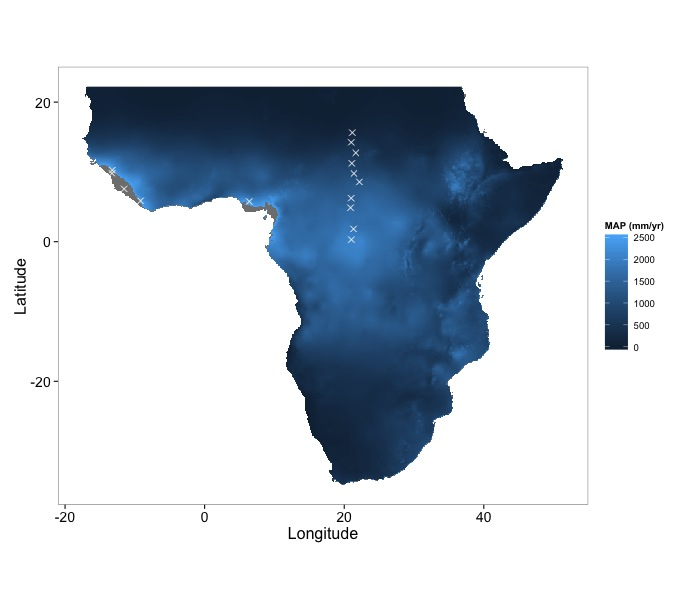
\includegraphics[height=.6\textheight]{images/cool1.jpeg}
\end{center}
\end{frame}
% --------------------------------------------------------------

\begin{frame}[fragile]
\frametitle{Demo gallery}
Hayward Godwin, \footnotesize{\url{http://www.psychwire.co.uk/2011/04/further-adventures-in-visualisation-with-ggplot2/}}
\begin{center}
  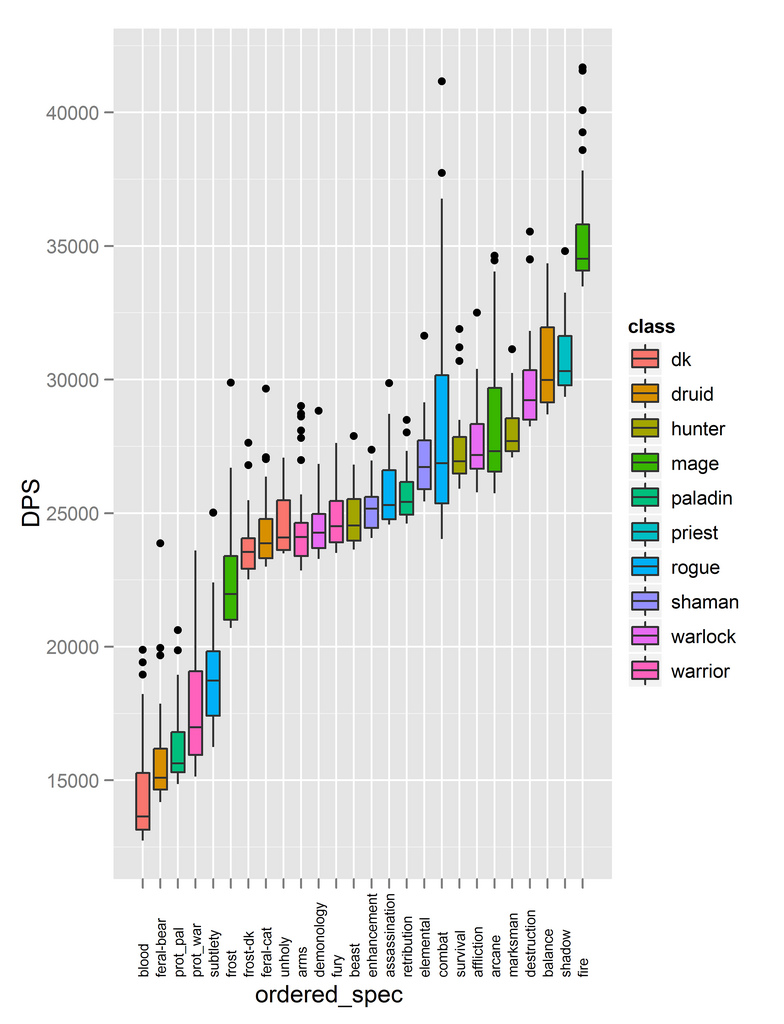
\includegraphics[height=.6\textheight]{images/cool2.jpg}
\end{center}
\end{frame}
% --------------------------------------------------------------

\begin{frame}[fragile]
\frametitle{Demo gallery}
Christophe Ladroue, \footnotesize{\url{http://chrisladroue.com/2012/02/polar-histogram-pretty-and-useful/}}
\begin{center}
  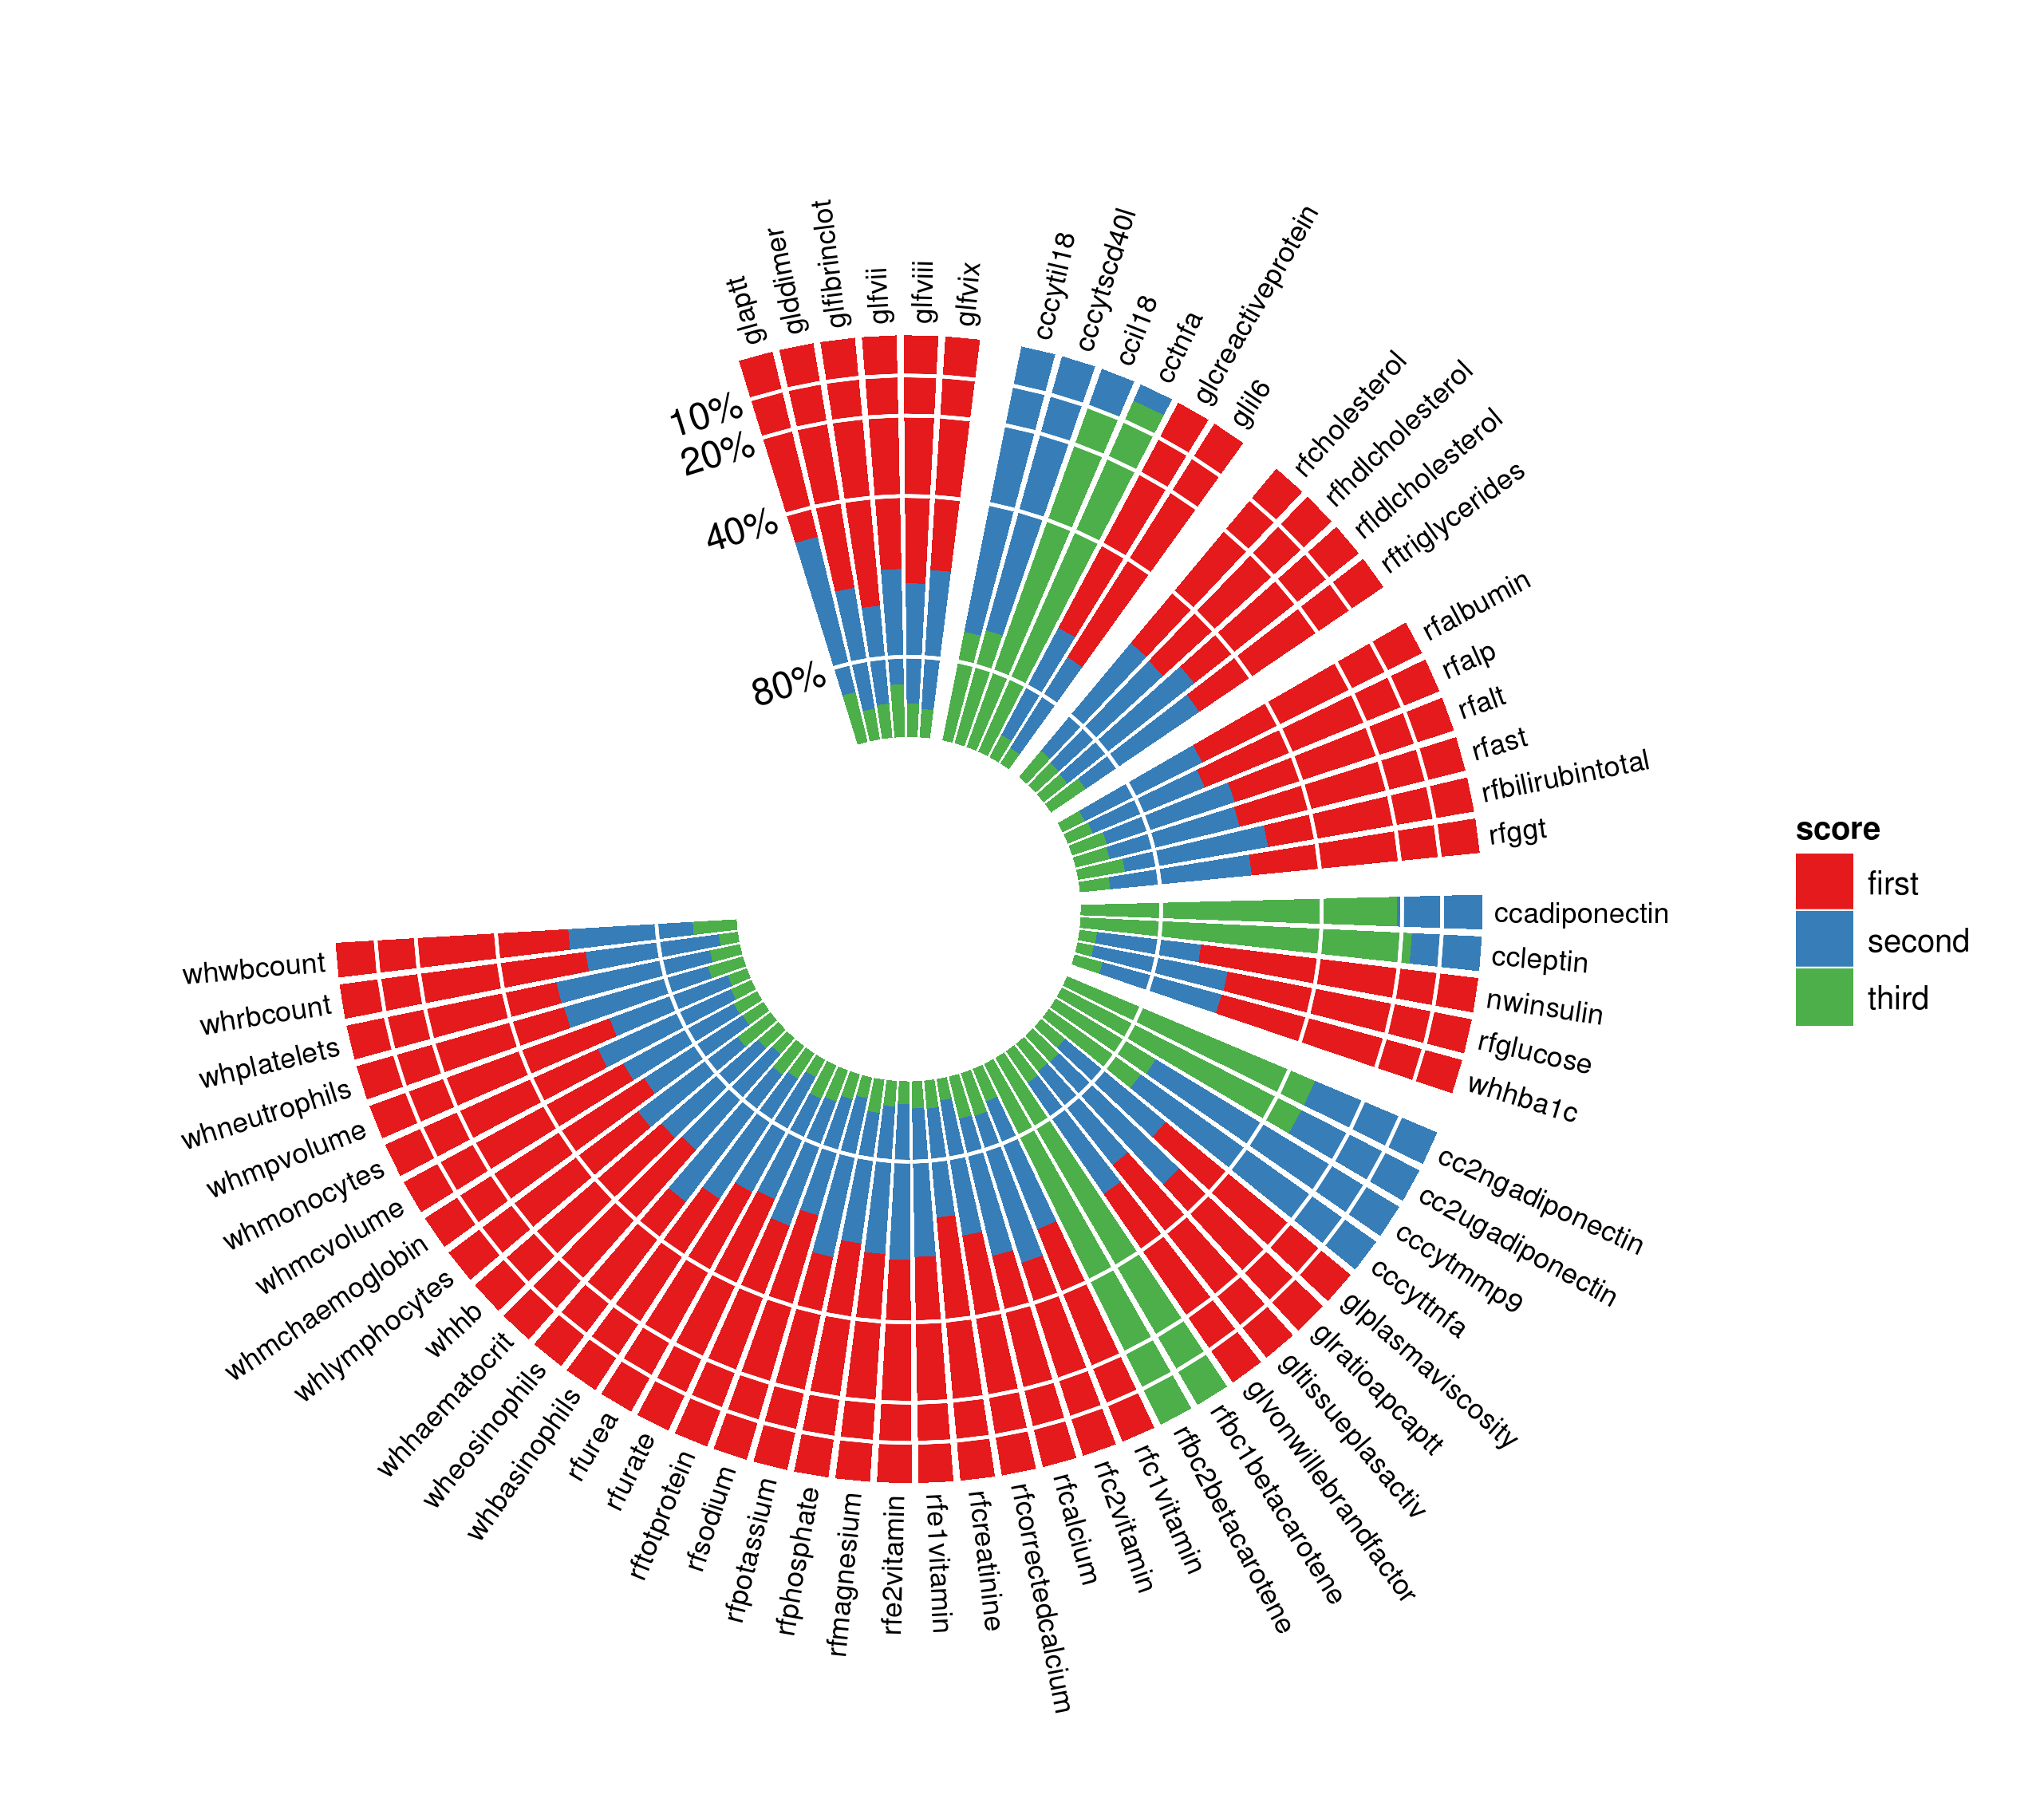
\includegraphics[height=.6\textheight]{images/cool3.png}
\end{center}
\end{frame}
% --------------------------------------------------------------

\begin{frame}[fragile]
\frametitle{Demo gallery}
Siguniang's blog, \footnotesize{\url{http://siguniang.wordpress.com/2011/04/17/mandelbrot-set-in-r/}}
\begin{center}
  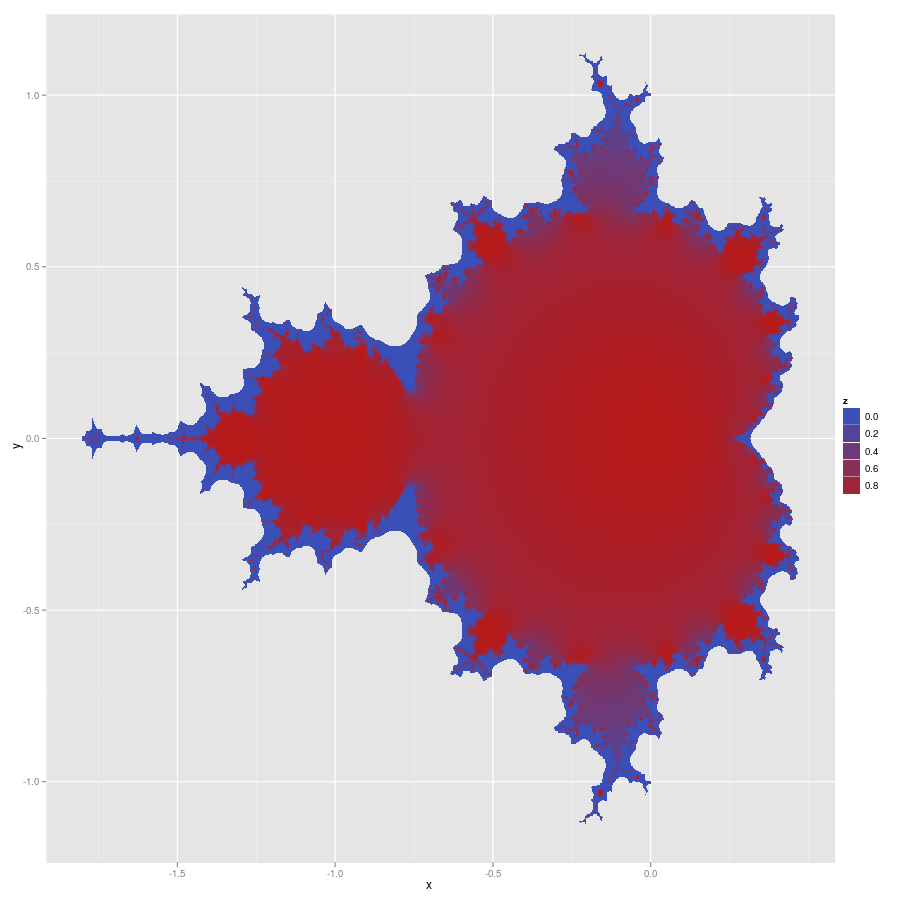
\includegraphics[height=.6\textheight]{images/cool4.png}
\end{center}
\end{frame}
% --------------------------------------------------------------

\begin{frame}[fragile]
\frametitle{Demo gallery}
Tony Hirst, \footnotesize{\url{http://blog.ouseful.info/2012/03/14/plotting-latitude-and-longitude-with-ggplot-map-projections-in-r/}}
\begin{center}
  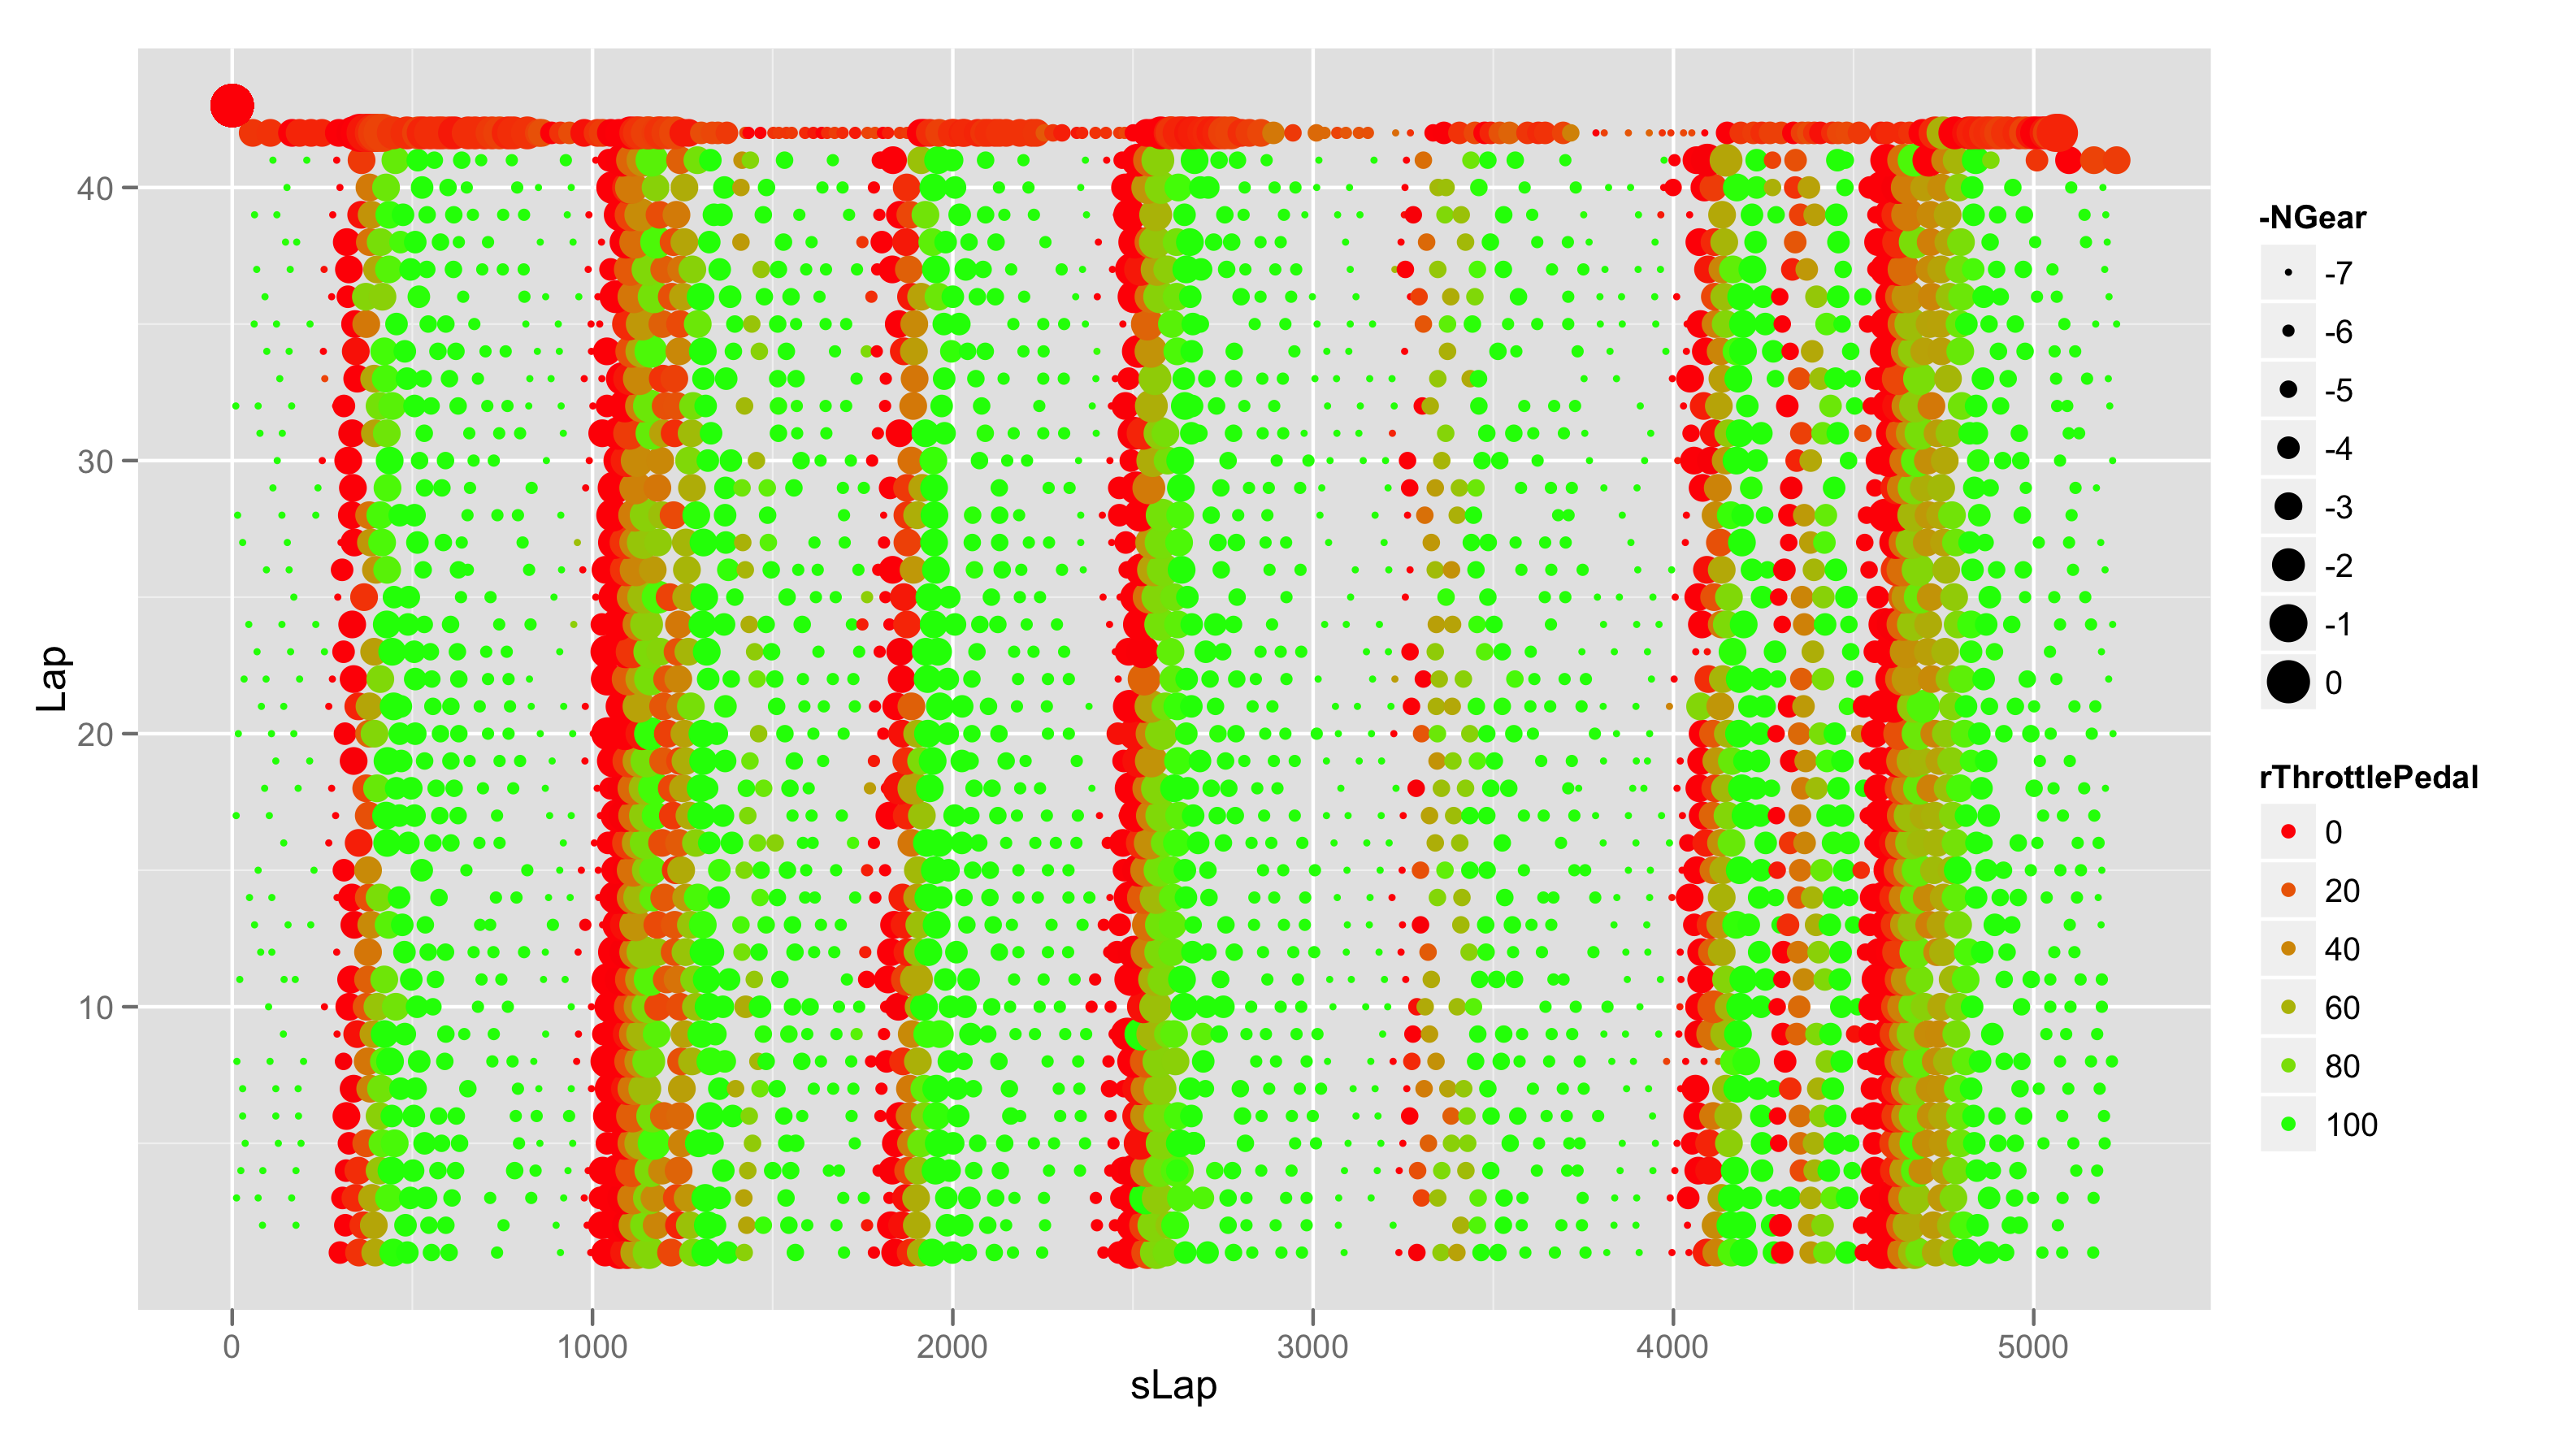
\includegraphics[height=.6\textheight]{images/cool5.png}
\end{center}
\end{frame}
% --------------------------------------------------------------
\end{document}
